走行ロボットの正面図と俯瞰図:
\begin{figure}[h]
    \begin{minipage}{0.48\linewidth}
        \centering
        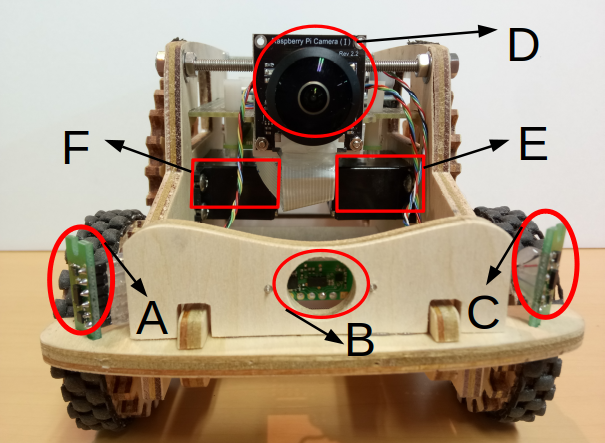
\includegraphics[width=0.9\linewidth]{robot1.jpg}
        \caption{正面図}
    \end{minipage}
    \begin{minipage}{0.48\linewidth}
        \centering
        \includegraphics[width=0.9\linewidth]{robot2.jpg}
        \caption{俯瞰図}
    \end{minipage}
\end{figure}

\begin{figure}[h]
        \centering
        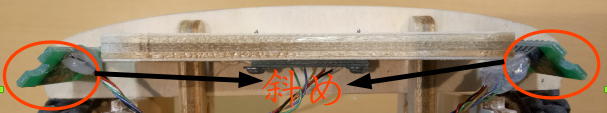
\includegraphics[width=1.0\linewidth]{robot4.jpg}
        \caption{左右のセンサー角度表示}
\end{figure}


A:右の距離センサー;B:中央の距離センサー;C:左の距離センサー;D:カメラ(使っていない);E:右モーター;F:左モーター;制御システム:ラズパイ;左右センサー角度:45\degree;ロボット幅:13.5;ロボット長さ:20.2;ロボット高さ:12.2;



今回使っているのは4輪木造走行ロボットである,人間や昆虫の走行特徴に近似するため,左右の車輪は左右のモーターで独自に制御して,超信地旋回できるようになる.tof距離センサーが赤外線の反射で距離を測るので,超音波より測る範囲が狭いけど,体積が小さく,精度が高くて,複数ロボットの場合,ロボット同士間の妨害も減少できる.

